\documentclass{article}

% if you need to pass options to natbib, use, e.g.:
%     \PassOptionsToPackage{numbers, compress}{natbib}
% before loading neurips_2019

% ready for submission
% \usepackage{neurips_2019}

% to compile a preprint version, e.g., for submission to arXiv, add add the
% [preprint] option:
    % \usepackage[preprint]{neurips_2019}

% to compile a camera-ready version, add the [final] option, e.g.:
\usepackage[final]{neurips}

% to avoid loading the natbib package, add option nonatbib:
    % \usepackage[nonatbib]{neurips_2019}
\usepackage{multicol}
\usepackage{float}
\usepackage[center]{caption}

\usepackage[utf8]{inputenc} % allow utf-8 input
\usepackage[T1]{fontenc}    % use 8-bit T1 fonts
\usepackage{hyperref}       % hyperlinks
\usepackage{url}            % simple URL typesetting
\usepackage{booktabs}       % professional-quality tables
\usepackage{amsfonts}       % blackboard math symbols
\usepackage{nicefrac}       % compact symbols for 1/2, etc.
\usepackage{microtype}      % microtypography
\usepackage{graphicx}
\usepackage{amsmath}
\usepackage{xepersian}

\settextfont{XB Yas.ttf}

\title{تکلیف شماره 5
 - 
 \lr{Consensus}}


% The \author macro works with any number of authors. There are two commands
% used to separate the names and addresses of multiple authors: \And and \AND.
%
% Using \And between authors leaves it to LaTeX to determine where to break the
% lines. Using \AND forces a line break at that point. So, if LaTeX puts 3 of 4
% authors names on the first line, and the last on the second line, try using
% \AND instead of \And before the third author name.

\author{%
  امیرحسین مهدی‌نژاد\\
  شماره دانشجویی 810800058\\
  \texttt{mahdinejad@ut.ac.ir} \\
  % examples of more authors
  % \And
  % Coauthor \\
  % Affiliation \\
  % \texttt{email} \\
  % \AND
  % Coauthor \\
  % Affiliation \\
  % Address \\
  % \texttt{email} \\
}

% create title (includes both anonymized and non-anonymized versions)
% \providecommand{\@makepertitle}{}
% \newcommand{\makepertitle}{%
%   \vbox{%
%     \hsize\textwidth
%     \linewidth\hsize
%     \vskip 0.1in
%     \toptitlebar
%     \centering
%     {\LARGE\bf \@title\par}
%     \bottomtitlebar
%       \def\And{%
%         \end{tabular}\hfil\linebreak[0]\hfil%
%         \begin{tabular}[t]{c}\bf\rule{\z@}{24\p@}\ignorespaces%
%       }
%       \def\AND{%
%         \end{tabular}\hfil\linebreak[4]\hfil%
%         \begin{tabular}[t]{c}\bf\rule{\z@}{24\p@}\ignorespaces%
%       }
%       \begin{tabular}[t]{c}\bf\rule{\z@}{24\p@}\@author\end{tabular}%
%     \vskip 0.3in \@minus 0.1in
%   }
% }

\begin{document}


\begin{minipage}{0.1\textwidth}% adapt widths of minipages to your needs

\includegraphics[width=1.1cm]{Photos/UT_logo.png}
\end{minipage}%
\hfill%
\begin{minipage}{0.9\textwidth}\raggedleft
دانشکده فنی، دانشگاه تهران\\
سیستم‌های توزیع شده - 
آذر
ماه 1400\\
\end{minipage}
% \end{}

\makepertitle

% ----------------------------------------------------------------------

% \begin{abstract}
%  این بخش از یک پاراگراف تشکیل شده است که توضیحاتی کلی در مورد مساله و راه حل شما ارائه می‌دهد.
% \end{abstract}
\begin{multicols}{2}
\section{}
پروسه‌های یک و دو
\lr{faulty}
هستند. پروسه‌ی ۱ فقط به ۲ پیام می‌دهد و از کار می‌افتد. پروسه‌ی ۲ بعد از ارسال پیام به ۱ و ۳ در راند دوم از کار می‌افتد.
لذا درخت این پروسه‌ها کامل نمی‌شود ولی درخت پروسه‌های دیگر قابل بررسی است.
\begin{figure}[H]
    \centering
    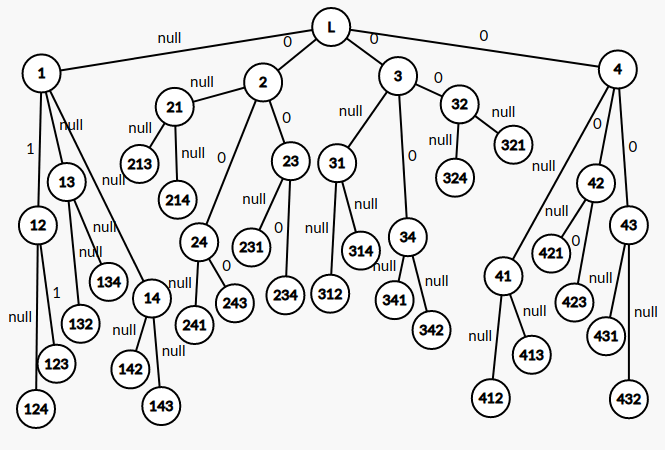
\includegraphics[width=0.99\linewidth]{Photos/HW5/p3.png}
    \caption{
    درخت پروسه‌ی سوم
    }
    \label{fig:my_label}
\end{figure}
\begin{figure}[H]
    \centering
    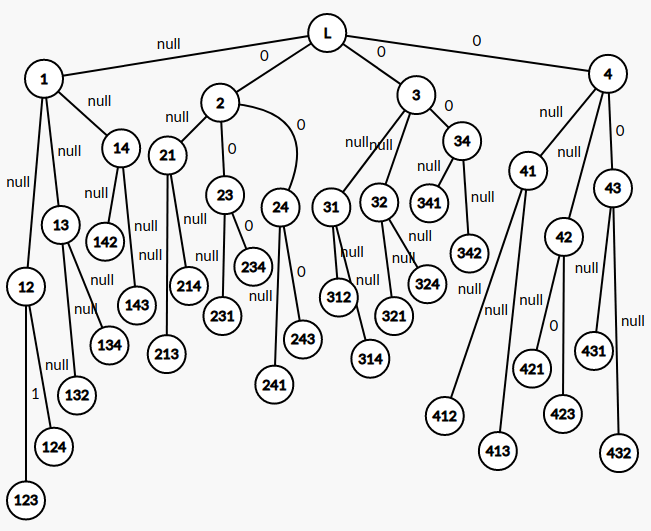
\includegraphics[width=0.99\linewidth]{Photos/HW5/p4.png}
    \caption{
    درخت پروسه‌ی چهارم
    }
    \label{fig:my_label}
\end{figure}
در مراحل ۲ به بعد، اطلاعات را با واسطه دریافت می‌کنیم لذا نقش نودهای دیگر اینجا تعیین‌کننده است. عدد ۳۲ در این گراف یعنی از ۲ شنیدیم که نظر ۳ چی بود و به همین ترتیب عدد ۲۳۴ یعنی از ۴ با واسطه شنیدیم که ۳ از ۲ چی شنید. \\
پس اگر پروسه‌ای
\lr{fail}
شد و پروسه‌ی دیگری قبل‌تر نظر آن را فهمیده بود، به نمایندگی در اختیار بقیه قرار می‌دهد.

در نهایت با توجه به برگ‌های درخت (۳تا صفر، ۱ یک و بقیه
\lr{null})
تصمیم
\lr{abort}
می‌شود. \\
\rule{\linewidth}{1pt}
\section{}
\subsection{هفت نود، دو فالت، دو راند}
با در نظر گرفتن نودهای ۶ و ۷ به عنوان نودهای خطاکار، اگر مقدار آن‌ها ۰ باشد ولی ۱ اعلام کنند، همچنین مقادیر نودهای ۱ و ۲ یک بوده و نودهای ۳، ۴ و ۵ صفر باشند، خواهیم داشت:
\begin{figure}[H]
    \centering
    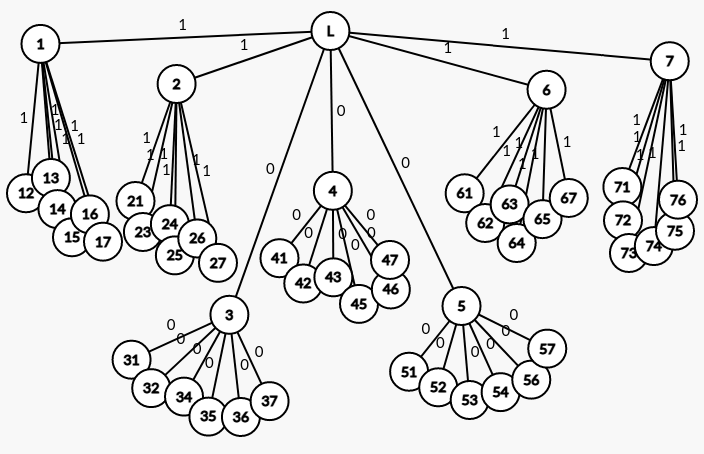
\includegraphics[width=0.99\linewidth]{Photos/HW5/p6.png}
    \caption{
    درخت پروسه‌ی ششم
    }
    \label{fig:my_label}
\end{figure}
به همین صورت پروسه‌های دیگر نیز دچار تصمیم نادرست می‌شوند.
همان‌طور که از شکل برمی‌آید، تصمیم نهایی (نظر اکثریت) ۱ است در صورتی که طبق
\lr{Validity}
نودهای
\lr{Non-Faulty}
باید روی ۰ به جمع‌بندی می‌رسیدند.\\
پیش‌تر نیز اشاره شده بود که برای \lr{f}
خطا نیاز به \lr{f+1}
راند داریم.
\subsection{شش نود، دو فالت، سه راند}
فرض کنیم پروسه‌های ۲ و ۳ نظر اولیه‌ی صفر داشته ولی
\lr{Faulty}
باشند. اگر نظر بقیه‌ی نودها را یک فرض کنیم، تصمیم نهایی باید ۱ شود.\\
اگر این نودها اطلاعات غلط در مورد پروسه‌های ۱ و ۶ در اختیار بقیه قرار دهند، در گره ۱۲ یعنی ۲ از ۱ چه پیامی گرفته، مقدار صفر را بدهد در صورتی که یک دریافت کرده بود. به همین ترتیب ۱۳ صفر، ۶۲ و ۶۳ نیز صفر شوند.

حال اگر از همان نودها ۱ و ۶ خطاکار باشند و به پروسه‌های ۲ و ۳ مقدار صفر اعلام کنند، این اطلاعات غلط باعث صفر شدن ۱۲، ۱۳، ۶۱ و ۶۳ خواهد شد.
\begin{figure}[H]
    \centering
    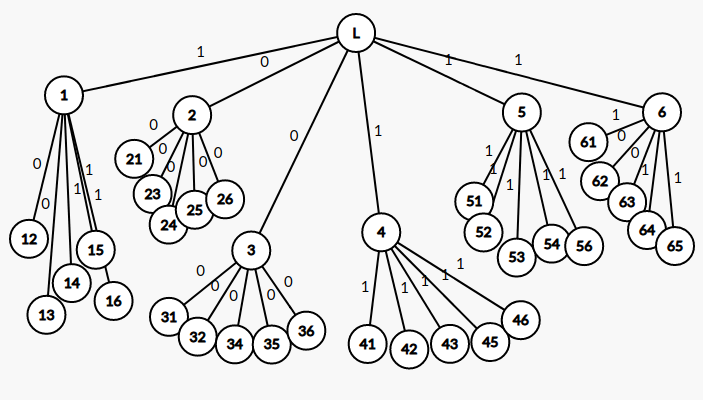
\includegraphics[width=0.99\linewidth]{Photos/HW5/same.png}
    \caption{
    درخت هر دو حالت مذکور
    }
    \label{fig:my_label}
\end{figure}
به دو حالت یکسان ولی با تصمیم نهایی متفاوت برای یک نود رسیدیم.\\
\rule{\linewidth}{1pt}
\section{}
شرط
\lr{Validity}
بیان می‌کند که اگر همه‌ی پروسه‌ها با یک مقدار شروع کنند، باید بر همان مقدار به اجماع برسند. این شرط در حالت وجود
\lr{Byzantine Failure}
به این صورت تغییر خواهد کرد که اگر همه‌ی پروسه‌های غیرخطاکار با یک مقدار شروع کنند، همان مقدار تصمیم نهایی خواهد بود.

می‌دانیم اگر شرایط مسئله برقرار باشد، الگوریتم
\lr{EIGByz}
در نهایت نظر نودهای خطادار را نادیده خواهد گرفت چون برای
\lr{Byzantine Failure}
طراحی شده است. پس اگر
\lr{Stop Failure}
داشته باشیم نیز می‌توان مثلا مقداری پیشفرض برای نودهای از کار افتاده در نظر گرفت و مسئله را معادل با خطاکار بودن نودها فرض کرد.

در این‌صورت می‌توان گفت اگر این الگوریتم قادر به حل مشکل
\lr{Stop}
نباشد انگار قادر به حل
\lr{Byzantine}
نیز نبوده است.
\end{multicols}
\end{document}
